% !TeX root = ../main.tex
% Add the above to each chapter to make compiling the PDF easier in some editors.

\chapter{System Design - DARVAH Proposal}\label{chapter:systemdesign}

In this chapter, we propose a dialogue framework for NLP applications implementing conversation flows, providing humorous responses via dialogue interfaces as specified in Chapter \ref{chapter:implementation}. The interfaces enable a dialogue system to communicate with the environment via software and hardware. The dialogue system comprises a feedback loop orchestrated as a set of states which allow Natural Language Generation and information extraction. Further, we elaborate on the proposed architecture. \par

\section{DARVAH Framework}\label{section:darvah}

\acrshort{darvah} system is a loop comprising five stages:
\begin{enumerate}
     \item \( D\) stands for "deduce" and is a state that decides whether to generate either humorous or conventional response.
     \item \( A_s\) stands for "assess" and is a state that selects an appropriate humour type according to available user data.
     \item \( R\) stands for "render" and is a state that produces a humorous text for reply given the selected type.
     \item \( V\) stands for "validate" and is a state that validates the generated response using emotion recognition feedback given positive or negative emotions experienced by the interlocutor.
     \item \( A_t\) stands for "attune" and is a state that adjusts the humour types scores of the given interlocutor.
\end{enumerate}
In this section, we clarify the roles and functioning of each module inside the dialogue system. Figure \ref{fig:darvah} shows a general structure of the proposed system. \par

\begin{figure}[htpb]
  \centering
  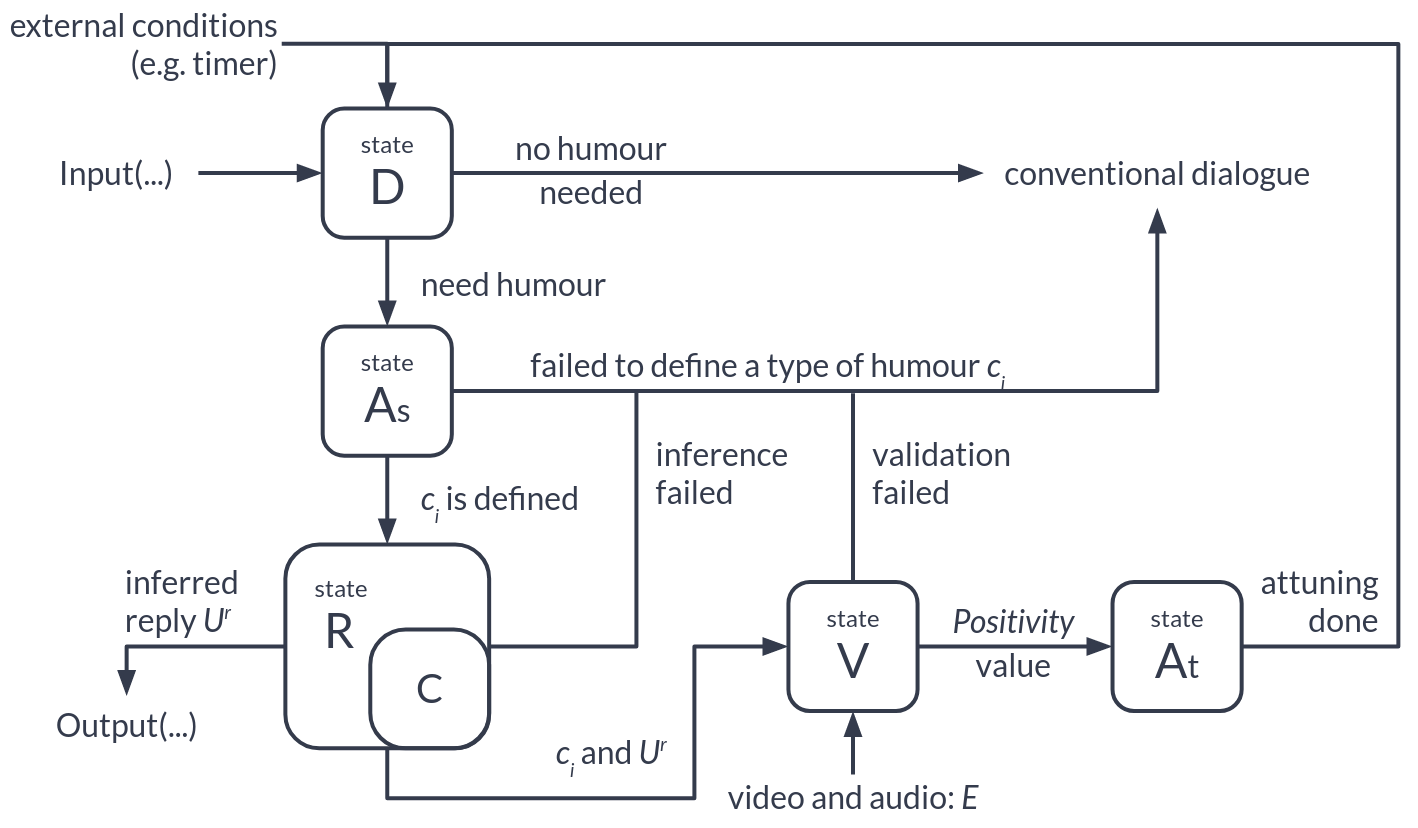
\includegraphics[width=0.8\textwidth]{figures/darvah.png}
  \caption{DARVAH system with the five main stages} \label{fig:darvah}
\end{figure}

\subsection{Deducing State \texorpdfstring{\( D\)}{D}}\label{subs:D}

To conduct a successful verbal exchange in a natural language, the Dialogue System requires capabilities to recognise whether the actual input is intelligible and entails an anticipated answer. The system makes a choice either to proceed with the ongoing conversation or to start a new one. In our case, this stage becomes the precursor to the humour generation process. Therefore, besides evaluating whether the input is relevant, the module has to answer a particular question: “Does the current state of the conversation prompt to pursue a humorous follow-up rather than a humourless one?” – i.e. to deduce if the conversation flow provides any immediate potential for a comical response (we denote this module by \( D\) which stands for “deducing/deciding”). It is important to note that we do not confine the module’s to exclusively natural language utterances as it is beneficial to incorporate other variables, e.g. computer vision to capture the emotion cues expressed by a conversational partner or other internal signals of the Dialogue System. \par
    
To illustrate how the module makes a decision, we will consider the following situation. Let’s assume two possible examples. Firstly, we could derive the condition to trigger the humour generation process via visual or audial cues prediction, such as negative emotion recognition result. This approach constitutes an active method of entering the DARVAH flow. In contrast, a passive approach presumes that users will be asking for a humorous response directly, for example:

\( U_{t-1}^{i}\): Please, tell me a joke

\( U_t^r\): Why are robots shy? Because they have hardware and software but no underwear.
    
where \( U_{t-1}^{i}\) is the utterance at the dialogue time step \( t-1\) which is the verbal input we received from the interlocutor \( I_i\). Considering the system produces a response at the current dialogue time step \( t\), \( U_{t}^{R}\) is the utterance produced by the robot at the current step. \par

Another possible valid approach is to randomly proceed with the humour generation process, to introduce an element of spontaneity to the Natural Language conversation, which often occurs in verbal interaction between humans. \par

In case module D does not decide to proceed with a humorous follow-up, it makes the dialogue system transition to the conventional dialogue states until the next time the decision process triggers. \par

\subsection{Assessing State \texorpdfstring{\( A_s\)}{As}}\label{subs:As}

If module \( D\) decides to proceed with a humorous follow-up, the system will activate the next module – \( A_s\). This module assesses which type of humour to utilise based on available user data. The Dialogue System data structures contain information about the current and previous interlocutors and associations between them and the joke types (see Ch. x). To choose a joke type to generate a humorous response subsequently, \( A_s\) introduces and uses the information about the likeability of each joke type defined as affinity scores. This process is not trivial since it has to take into account further joke types score adjustments happening in the module \( A_t\). To clarify the process, let’s consider the following example of the possible affinity values provided in Table \ref{table:1}. \par
    
\begin{table}[htpb]
\centering
\begin{tabular}{ |l|l l l l l l l|  }
    \hline
    \multicolumn{8}{|c|}{Affinity Scores} \\
    \hline
    ... & \( c_1\) & \( c_2\) & ... & \( c_j\) & ... & \( c_{n-1}\) & \( c_n\) \\
    \hline
    \( I_{i-1}\) & 5 & 5 & ... & 8 & ... & 5 & 0 \\
    \( I_{i}\) & 5 & 10 & ... & 15 & ... & 20 & 5 \\
    \( I_{i+1}\) & 10 & 20 & ... & 5 & ... & 0 & 0 \\
    \hline
    \end{tabular}
\caption{Example affinity scores before the assessment}
\label{table:1}
\end{table}
    
Where \( c_j\) is a joke category (or type), \( j \in [1, n]\) and \( I_i\) is a current interlocutor \( i\). The score scale is an integer scale with a step of 1 with each score \( s_ij \in [0, 100]\). \( S_i=\{s_1, s_2,..., s_n\}\) is then a vector of affinity scores that belongs to the interlocutor \( I_i\). \par

At the current step in module \( A_s\), we require a heuristic to choose the next type of joke. Obviously, by choosing one with the maximum score, we are reinforcing only a single type of jokes until its complete saturation. If it is the case, we cannot select any other type, and the interlocutor will not be able to judge whether he or she prefers any other joke more. Therefore, the situation requires a more creative approach to resolve the saturation and flexible choice issues. To address the challenge, we proposed the following simple choosing strategy:
\[ c_j=Assess(S_i)\]
where 
$$
Assess(S_i)=
    \begin{cases}
        choice(C_j^+), & \text{if $Validate(E_{t-2}^{i}[m]) \geq 1$}\\
        choice(C_j^-), & \text{if $Validate(E_{t-2}^{i}[m]) < 0$}\\
    \end{cases}
$$
where \( Validate(E_{t-2}^{i}[m])\) is the validation result (defined further in Section \ref{subs:At}) from the previous run of the DARVAH loop. Vector \(C_j^+\) contains all types for which values from \(S_i\) are bigger or equal to \( mean(S_i)\) and vector \(C_j^-\) contains all values all types for which values from \(S_i\) are less than \( mean(S_i)\). \(choice(C_j)\) is a random choice function that generates a sample from given array of number assuming any kind of a probability distribution over the values, for example, a uniform distribution.

Let's consider the current scores \( S_i=\{5, 10,..., 15,..., 20, 5\}\) for interlocutor \( I_i\). Assuming that 
$$ mean(S_i) = \frac{1}{N} \sum_{n=1}^{N} S_in = 11$$
and \( Validate(E_{t-2}^{i}[m])\) = 1, 
\[ Assess(S_i)=choice(c_j, c_{n-1}, ...)\]

If for some reason \( A_s\) fails to choose any type, it hands-over control to the conventional dialogue. \par

\subsection{Rendering State \texorpdfstring{\( R\)}{R}}\label{subs:R}

After module \( A_s\) selected the joke type, module \( R\) assumes control and proceeds with the \acrfull{nlg} task. This module is the principal stage of the humour-generation process and provides an interface to a \acrlong{nlg} sub-module – the Comedian. \( R\) can choose between proactive and reactive response rendering. We distinguish between these two kinds of humorous language generation due to the following reasoning. \par

The proactive response usually comprises a storytelling bit, when a group of people listen to the entertainer until he finishes. The performer narrates the bits of monologue, which are similar in rhythm, to build up the story. And at the end of the monologue, there is usually a culmination that takes an unexpected turn. In contrast, reactive response assumes active engagement in a conversation from both sides. The case is that when one conversation partner makes a remark, the other makes another one in response. Thus, this type of humour demonstrates more improvised features. For instance, stand-up is primarily a proactive type of comedy, while puns are often reactive. \par

Therefore, to be able to choose either proactive or reactive response rendering, we propose a decision-making function \( F_d(c_j, U_{t-1}^i) \in \{True, False\}\). A simple example of such a function could be:
$$
F_d(c_j, U_{t-1}^i)=
    \begin{cases}
        True, & \text{if $\exists c_j \in \{c_1, ..., c_n\}: Similarity(c_j, Triple(U_{t-1}^i)) \geq 1$}\\
        False, & \text{otherwise}
    \end{cases}
$$
where \( c_j=Assess(S_i)\) is one of the humour categories, 
\[ Triple(U)=\{Subject(U), Predicate(U), Object(U)\}\] 
is a function which produces triple from sentence \( U\) and 
$$ 
Similarity(c, Triple(U))= \sum_{k=1}^{3} sim(c, Triple(U)_k) \in [0, 3]
$$
is a function that calculates a sum of semantic similarity \(sim(x, y)\) between \( c\) and \( Subject(U)\), \( Predicate(U)\) and \( Object(U)\). \par

A positive or negative decision will affect the rendering process in the following way. To obtain a response, we will pass only the selected type of humour if the decision was to use proactive humour (\( F_d(c_j, U_{t-1}^i) = False\)). Otherwise, we will also pass the interlocutor's input utterance \( U_{t-1}^i\):
$$
Render(c_j, U_{t-1}^i)=
    \begin{cases}
        Comedian(c_j, U_{t-1}^i), & \text{if $F_d(c_j, U_{t-1}^i) = True$}\\
        Comedian(c_j), & \text{otherwise}
    \end{cases}
$$
here, \( Comedian: {c_j, U^i} \mapsto U^r\) is a variadic function that represents the \acrshort{nlg} sub-module. The sub-module is a black-box abstraction over a humour-conditioned Language Model which creates humorous sentences and can represent any combination of rule-based production systems with \acrshort{dnn}-based systems. After module \( R\) obtained the utterance \( U_t^r\), the system outputs the response by the means of textual and/or speech interfaces. \par

\subsection{Validating State \texorpdfstring{\( V\)}{V}}\label{subs:V}

To validate the emotional response, we propose module \( V\) which recognises emotion patterns expressed by the interlocutor, for example, visual and audial cues. The module receives a set of emotions scores vectors \( E_t^i\) for interlocutor \( I_i\). These emotions can be separated into positive and negative ones. Therefore, we compare a sum of positive emotions scores against a sum of negative emotions scores for each vector \( E_t^i\) according to the following function:
$$
Positivity(E_t^i)=
    \begin{cases}
        1, & \text{if $\sum_{n=1}^{N} E_{t,n}^{i+} > \sum_{n=1}^{N} E_{t,n}^{i-}$} \\
        0, & \text{if $\sum_{n=1}^{N} E_{t,n}^{i+} = \sum_{n=1}^{N} E_{t,n}^{i-}$} \\
        -1, & \text{if $\sum_{n=1}^{N} E_{t,n}^{i+} < \sum_{n=1}^{N} E_{t,n}^{i-}$}
    \end{cases}
$$ \par
where N is the number of recognised emotions. \par

Then, for \( E_t^{i}\) - an array of \( m\) vectors \( E_t\):
\[ Validate(E_t^{i})=mode\{Positivity(E_{t,1}^{i}), Positivity(E_{t,2}^{i}),..., Positivity(E_{t,m}^{i})\}\]

When the validation module obtains the result, it passes the value to module \( A_t\).

\subsection{Attuning State \texorpdfstring{\( A_t\)}{At}}\label{subs:At}

When the system receives the validation result in module \( A_t\), it will add 1 point to the score if the interlocutor preferred the evaluated types of humour. For the types that interlocutor did not like, the module will subtract 1 point from the score. For example, if, for the selected type \( c_j\), \( Validate(E^{i}[m]\) equals to 1, \( A_t\) needs to increase the affinity score \( s_{ij}\) by 1 as per:
$$
Attune(S_i|c_j)=
    \begin{cases}
        s_{ij}=s_{ij}+1, & \text{if $Validate(E_t^{i})=1$} \\
        s_{ij}=s_{ij}, & \text{if $Validate(E_t^{i})=0$} \\
        s_{ij}=max(s_{ij}-1, 0), & \text{if $Validate(E_t^{i})=-1$}
    \end{cases}
$$ \par
Besides the current score adjustments, \( A_t\) performs value decay over time according to a decay multiplier parameter applied to each value based on the timestamp of the previous update to introduce the functionality to slowly forget humour preferences. This capability is convenient if we expect our interlocutors to interact with the robot again after a long period of time because the decay function will first discard the scores with lower values allowing the most favourite joke categories to persist longer.  

Given that the decay strategy can be arbitrary, we propose to define the parameter as a percentage of each score the system forgets over each preceding interval of time. Then, we calculate the number of intervals since the previous update of the scores and raise the decay multiplier to the power of the amount of the interval. Afterwards, updated affinity scores equal to each of them multiplied by the resulting value and rounded:
\[ S_i^{'} = round((1-p)^{\frac{t_now-t_prev}{T}}S_i)\]
where \( p\) is the decay parameter, \( T\) is the period in seconds, \( t_now\) is the current time, and \( t_prev\) is the time of the last update. Rounding function is the round half away from zero function as following:
\[ round(x)=sgn(x)\lfloor|x|+0.5\rfloor=-sgn(x)\lceil|x|-0.5\rceil\] \par

For example, let's set \( p=0.1\) which corresponds to 10\% decay and \( T = 86400 s\) which equals to 1 full day. Given that the last update for interlocutor \( I_{i-1}\) happened two days ago, the decayed scores will be:
\begin{multline*}
S_i^{'} = round(((1-0.1)^{\frac{2*86400}{86400}}(5, 5,..., 5,..., 5, 0)) = round(0.81(5, 5,..., 10,..., 5, 0)) \\ = (4, 4,..., 8,..., 4, 0)
\end{multline*} \par
    
Given values in Table \ref{table:1}, we provide the final scores adjustment result in Table \ref{table:2}.
    
\begin{table}[htpb]
\centering
\begin{tabular}{ |l|l l l l l l l| }
    \hline
    \multicolumn{8}{|c|}{Affinity Scores} \\
    \hline
    ... & \( c_1\) & \( c_2\) & ... & \( c_j\) & ... & \( c_{n-1}\) & \( c_n\) \\
    \hline
    \( I_{i-1}\) & 4 & 4 & ... & 8 & ... & 4 & 0 \\
    \( I_{i}\) & 5 & 10 & ... & 16 & ... & 20 & 5 \\
    \( I_{i+1}\) & 10 & 20 & ... & 5 & ... & 0 & 0 \\
    \hline
    \end{tabular}
\caption{Example affinity scores after the adjustment process}
\label{table:2}
\end{table}

After \( A_t\) finishes the score attuning process, state \( D\) becomes active again.

\section{The Comedian}

In this section, we would like to clarify the difference between proactive and reactive humorous \acrlong{nlg} tasks. Since we are employing a Language Model based on GPT-2 \acrlong{dnn} {model}, the following example illustrates the usage of this particular.

Because GPT-2 can accept from one to technically unlimited amount of tokens as an initial prompt to generate further tokens, it inherently represents a variadic function. This feature allows us to use the model as the Comedian submodule without any unique intermediate interfaces or combinations of separate Language Models for either proactive or reactive response generation tasks.

Let's consider the following toy problem. Given the model \( \mathcal{M}\) implementing the GPT-2 architecture and the dataset \( \mathcal{D}\) containing:
\begin{itemize}
    \item a single class: \( c_j = <|robot|>\)
    \item a single sentence: \( U = \)"Why are robots shy? Because they have hardware and software but no underwear."
\end{itemize}
which form a single data point:
\begin{itemize}
    \item<|robot|>Why are robots shy? Because they have hardware and software but no underwear.<|endoftext|>
\end{itemize}
we had trained \( \mathcal{M}\) on the dataset until it overfitted. Now, we would like to test how it performs in the \acrshort{nlg} task.

Case 1: Proactive response generation.

If we have set the input utterance to an empty value \( U_{t-1}^i = \)"" and run the response generation, we will obtain the following result:
\begin{enumerate}
    \item chosen class: \( c_j = <|robot|>\)
    \item input utterance: \( U_{t-1}^i = \)""
    \item decision-making function: \( F_d(c_j, U_{t-1}^i) = False\)
    \item rendering function: \( Render(c_j, U_{t-1}^i) = Comedian(c_j) = \mathcal{M}(c_j)\)
    \item response utterance: \( U_t^r = \mathcal{M}(<|robot|>) = \)"Why are robots shy? Because they have hardware and software but no underwear."
\end{enumerate}

Case 2: Reactive response generation.

If we have set the input utterance to a specific value \( U_{t-1}^i = \)"Why are robots shy?" and run the response generation, we would obtain the following result:
\begin{enumerate}
    \item chosen class: \( c_j =  <|robot|>\)
    \item input utterance: \( U_{t-1}^i = \)"Why are robots shy?"
    \item decision-making function: \( F_d(c_j, U_{t-1}^i) = True\)
    \item rendering function: \( Render(c_j, U_{t-1}^i) = Comedian(c_j, U_{t-1}^i) = \mathcal{M}(c_j, U_{t-1}^i)\)
    \item response utterance: \( U_t^r = \mathcal{M}(<|robot|>,\) "Why are robots shy?"\() = \)"Because they have hardware and software but no underwear."
\end{enumerate}

The main difference is that the model will incorporate the reactive input utterance (which can also be pre-processed into more sophisticated tokens before use) as a stronger prior for the generated tokens. This approach could be useful, for example, for a question-answering task such as riddle jokes. This style of humour represents riddles that ask a question as a premise for a humorous punch line for an answer.

\section{DARVAH Ontology}

In this section, we would like to mention our proposal to implement an ontology for the DARVAH framework.

Again, let's consider our example from Section \ref{section:darvah}. If we define a graph
\[G = (\{I, C\}, \{\{I_1, c_1\}, \{I_1, c_2\}, ..., \{I_i, c_j\},...\})\]
where \(\{I, C\}\) is a set of vertices, \(I\) is a set of all interlocutors and \( C\) is a set of all humour categories such that they form the nodes of the graph \( G\) , then we can assign a connection from each interlocutor to each type of humour \( \{I_i, c_j\}\). The scores \( s_{ij}\) will define the weight of the connection. Therefore, for interlocutor \( I_i\), \( S_i\) will denote all weights of all connections to all humour categories in the graph (see Figure \ref{fig:graph}). Using this approach, the \( Assess(S_i)\) function simply returns the humour node \( c_j\) with the corresponding connection weight \(r_{ij}\) (as per  affinity scores in Table \ref{table:1}):
\[ s_{ij}=r_{ij}(I_i \to c_j)=15\] 
while the \(Attune(S_i|c_j)\) function changes the weight of the connection (as per affinity scores in Table \ref{table:2}):
\[ r_{ij}(I_i \to c_j)=s_{ij}=16\]
This architecture is very convenient to use in a graph-based database and easily supports adding new types and interlocutors. Since it is possible support Neo4j database, thanks to this design decision, we can integrate the DARVAH ontology directly into Ravestate ontology.

\begin{figure}[htpb]
  \centering
  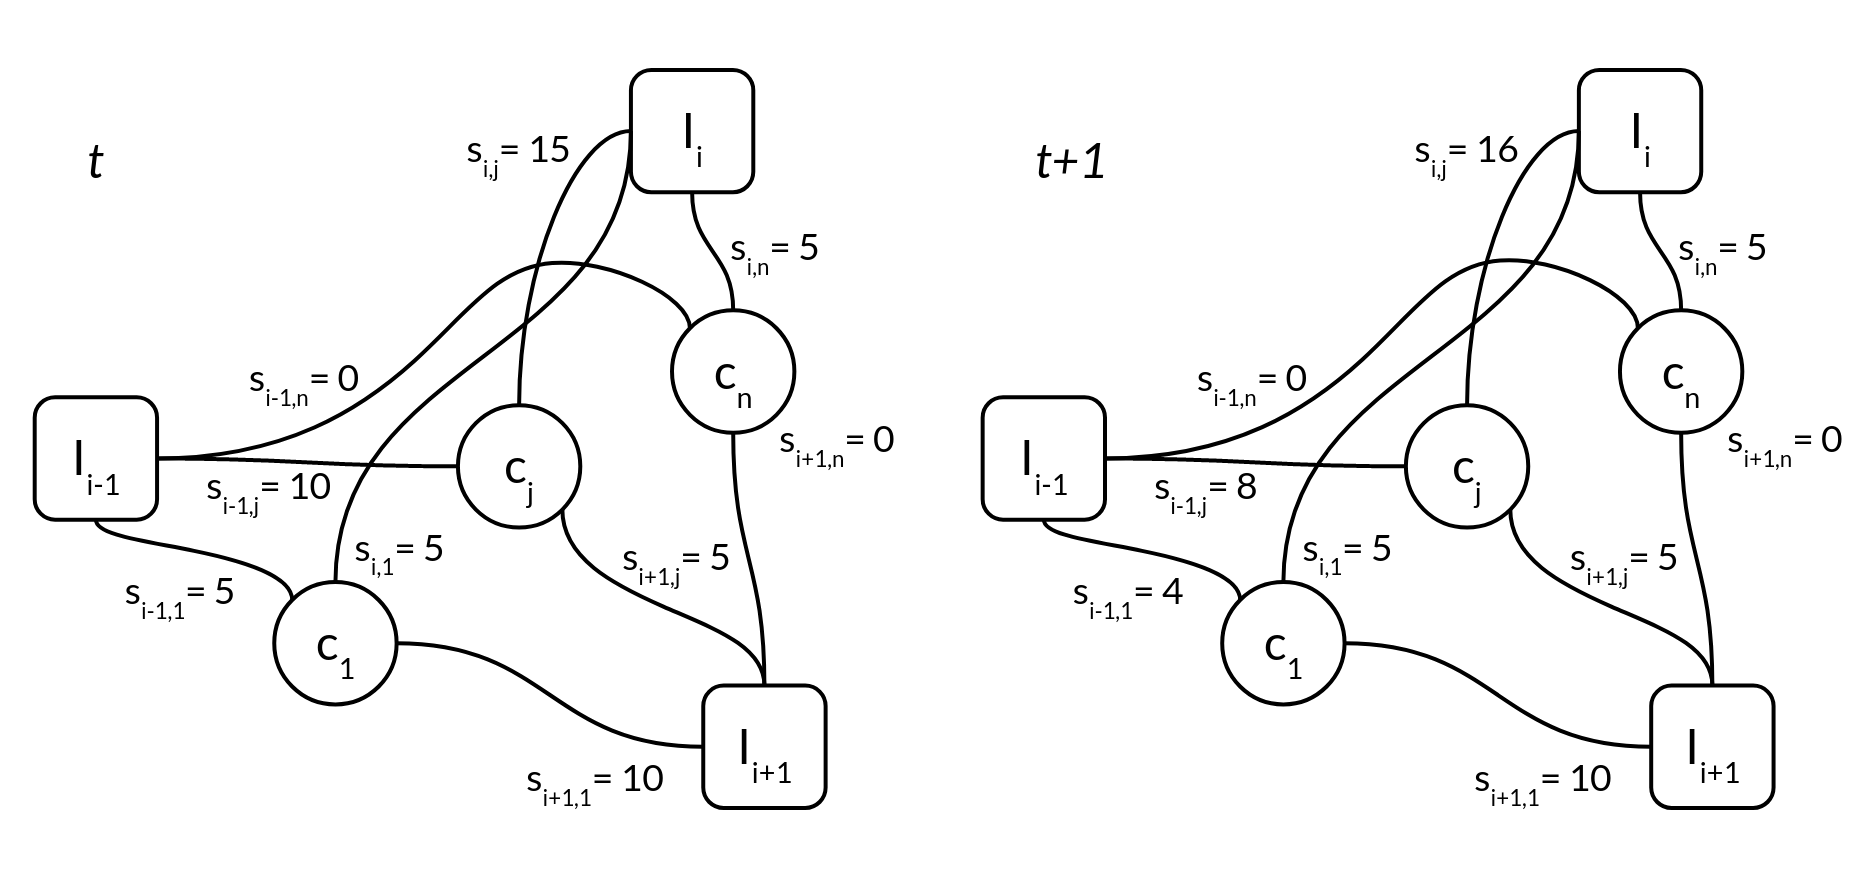
\includegraphics[width=1.0\textwidth]{figures/ontology.png}
  \caption{The ontology graph for DARVAH before and after attuning the scores.} \label{fig:graph}
\end{figure}

\section{Emotion Recognition Subsystem}\label{section:ers}

In this section, we discuss an approach to collecting and using emotion recognition data. Since it is unclear at which moment of system time we need to validate the emotion recognition data, we propose to continuously evaluate the input sources such as camera and microphone streams and access the recognition results as soon as we need them for the validation step. Therefore, we imagine the task of emotion recognition as a series of discrete steps where \acrshort{fer} and \acrshort{ser} run as two parallel processes (see Figure~\ref{fig:aer}).

\begin{figure}[htpb]
  \centering
  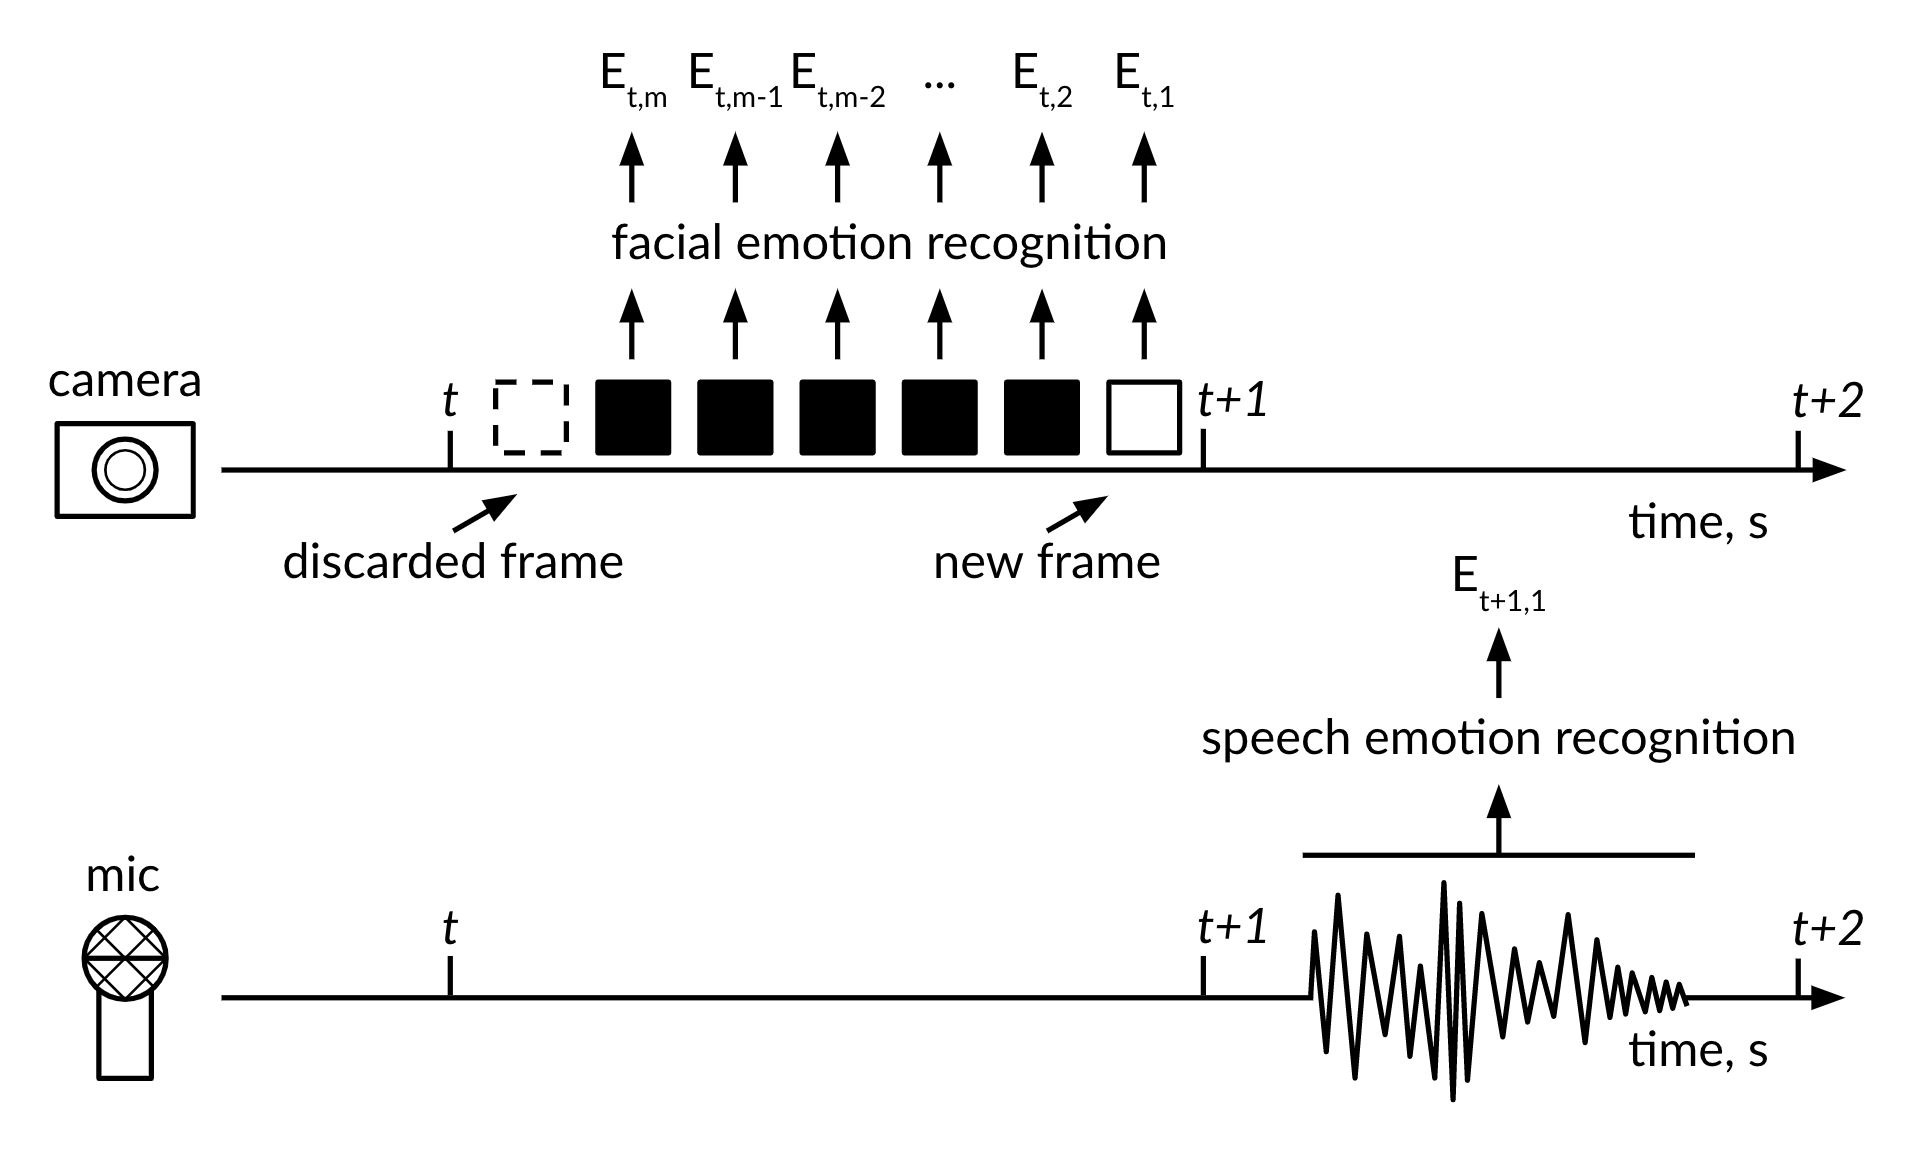
\includegraphics[width=0.9\textwidth]{figures/aer.png}
  \caption{The emotion recognition timeline for DARVAH.} \label{fig:aer}
\end{figure}

\subsection{Facial Emotion Recognition}

For the \acrshort{fer} task, we can enable our \acrlong{fer} to capture web camera video stream frame-wise and classify facial emotions based on each frame. Thus, the DARVAH framework can access the latest \( m\) results from the recognition subsystem at any moment of system time. At the time step \( t\), when state \(R\) has produced the response utterance \( U_t^r\), the validation state will receive:

\[ E_t^i = \{E_{t,1}^i, E_{t,2}^i,..., E_{t,m-1}^i, E_{t,m}^i\}\]

where \(m = f \times w\), \( f\) is the frequency of sampling and \( w\) is the window size. For the standard sampling \(f = 30 Hz\) (frames per second in the stream) rate and a window size \(w = 10 s \) (which is a sufficient size for most of the response utterances \( U_t^r\) to be perceived by the interlocutor \( I_i\)), \( E_t^i \) will contain m = 30 Hz * 10 s = 300 emotion score vectors.

As soon as the \acrshort{fer} module receives a new sample, it discards the oldest one according to first-in, first-out (FIFO) queue principle, such that the last added element is always the most recent recognition result. On the DARVAH side, we can access all of the queue elements as an ordered list.

\subsection{Speech Emotion Recognition}

To successfully perform the \acrshort{ser} task, we need to record the following spoken utterance \( U_{t+1}^i\) by the interlocutor. As soon as the robot is done vocalising the response \( U_t^r\), we can start the recording and finalise it as soon as the interlocutor stopped speaking. After the \acrshort{ser} module obtains the recording, it recognises the emotions in speech and outputs a single vector of the emotion scores which we denote by \( E_{t+1}^i \) given that the following utterance by the interlocutor \( I_i\) occurs in the next time step after the response \( U_t^r\). However, this circumstance means that state \( V\) can only utilise the \acrshort{ser} result when \acrshort{darvah} produces the next response at time step \( t+2\) because the previous execution of the DARVAH loop has already completed.
To resolve this discrepancy, we propose the following emotion combination rule:

$$ 
E_{t+2}^{i'} = \sum_{k=1}^{m}{\alpha E_{t+2,k}^i + \beta E_{t+1}^i}
$$

where \( \alpha \in [0, 1]\) and \( \beta \in [0, 1]\) are the weights for vectors \( E_{t+2,k}^i \) and \( E_{t+1}^i \) respectively, such that \( \alpha + \beta = 1\). At the next DARVAH time step \( t+2\), this rule allows the previous \acrlong{ser} result from interlocutor's input \( U_{t+1}^i\) to condition the next emotion evaluation \(Validate(E_{t+2}^{i})\).